\chapter{Estado del arte y fundamentos teóricos}

Antes de empezar a escribir código, se deben entender los conceptos fundamentales que permitirán llevar a cabo este trabajo.

Lo que se intenta mejorar utilizando Dagger es el ciclo completo de CI/CD de una aplicación. Por lo tanto, es fundamental definir los conceptos de \textit{Continuous Integration} y el \textit{Continuous Delivery}. Una vez se comprenda a qué se refieren esos términos, se podrán entender los métodos y tecnologías convencionales que permiten implementar dichos procesos. Será entonces cuando se pueda introducir Dagger, un método innovador para realizar \textit{pipelines}, el cual aporta muchas ventajas y se comparará con otras tecnologías disponibles en el sector.

\section{CI/CD}

CI/CD son las siglas de \textit{Continuous Integration}/\textit{Continuous Delivery}, o en casos más específicos, este último también se puedo conocer como \textit{Continuous Deployment}.

Se trata de un conjunto de pasos automatizados, utilizados en el desarrollo de software para llevar el código desde su implementación inicial hasta el despliegue de la aplicación. Estos pasos incluyen:

\begin{itemize}
  \item Integración de cambios en el código.
  \item La compilación de la aplicación con los cambios realizados.
  \item Realización de pruebas.
  \item Creación y publicación de imágenes de Docker y paquetes NPM.
  \item Despliegue de la aplicación (modelo \textit{push}\cite{push})
\end{itemize}

\subsection*{\textit{Continuous Integration}}

Se basa en la integración de código de manera constante, día a día, en un repositorio compartido por programadores. Cada uno de los programadores realiza cambios en el código y lo integra en el repositorio. Una vez se realizan cambios, estos deben pasar una serie de pruebas para que se incluyan definitivamente en el código fuente de la aplicación (Fig. \ref{ci}).

\begin{figure}
  \centerline{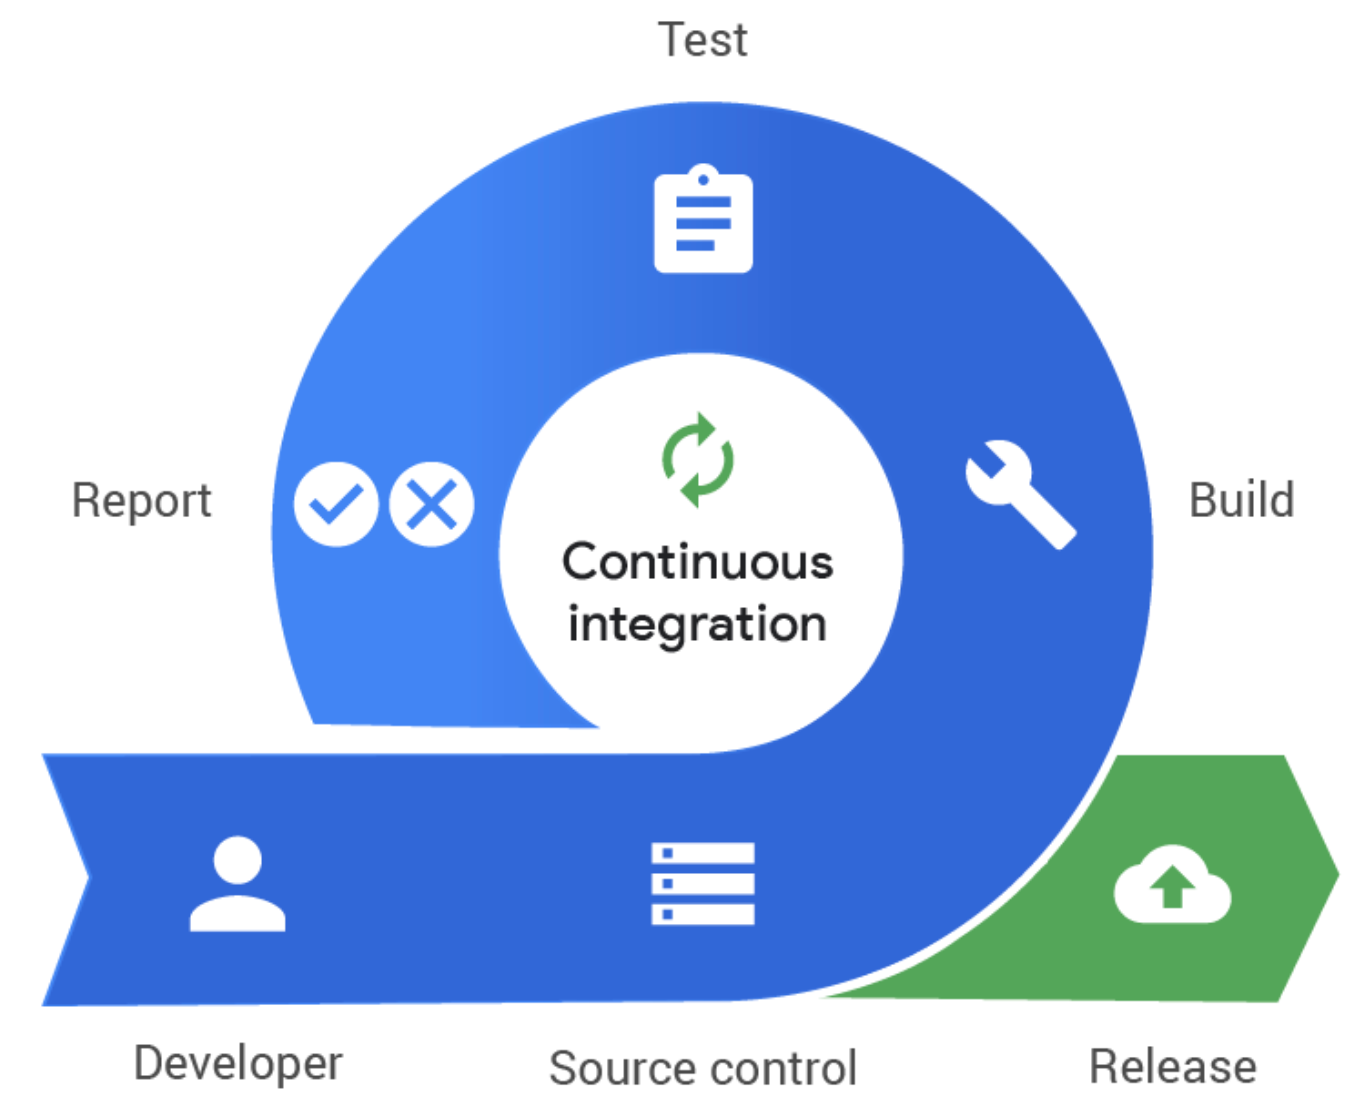
\includegraphics[width=10cm]{figuras/ci}}
  \caption{Proceso de integración continua.\cite{img.ci}}
  \label{ci}
\end{figure}

Desde hace años se utiliza un sistema de control de versiones para gestionar el código de cualquier proyecto. Este tipo de herramientas permite a un equipo controlar el estado del código en cada momento, siendo capaces de conocer el historial de los cambios realizados, saber quién ha hecho cada cambio y tener la capacidad de revertir alguna modificación en el caso de ser necesario. La herramienta de control de versiones más utilizada hoy en día, y la que se utiliza en este proyecto, es Git\cite{git}.

La integración de código en un repositorio no se trata simplemente de modificar una porción de un archivo y subirlo. El código debe ser probado antes de incluirlo completamente en el núcleo de la aplicación. Durante el proceso de integración continua, cada vez que se modifica algo de código, se debe:

\begin{itemize}
  \item Construir la aplicación.
  \item Pasar pruebas de funcionalidad.
  \item Pasar a través de un análisis del propio código (\textit{linting}).
  \item Reportar cualquier error en el caso de que exista.
\end{itemize}

Todo lo anterior se debe realizar de manera automatizada, con el fin de integrar el código modificado en la aplicación lo más rápido posible.

\section{Métodos convencionales}

Como cabe esperar, los pasos mencionados anteriormente que forman parte de la integración continua van a depender del tipo de aplicación que se esté construyendo, y de las tecnologías que se estén utilizando. Además, esta secuencia de acciones pueden incluir unos pocos comandos en trabajos o proyectos sencillos, o necesitar varios \textit{scripts} complejos en el caso de aplicaciones más avanzadas. Por lo tanto, es necesario tener una herramienta que permita realizar los pasos mencionados anteriormente, sin la necesidad de memorizar o saber a ciencia cierta cada uno de los comandos o scripts que hay que ejecutar para comprobar que el código de la aplicación es correcto.

Para ello existe \texttt{make}\cite{make}, una aplicación de línea de comandos que permite definir bloques de comandos o reglas, aportando a cada bloque un nombre u objetivo que se pretende obtener ejecutando dicha regla. Se suele crear un archivo llamado \texttt{Makefile} para definir todas las reglas que se precisen.

\begin{lstlisting}[language=make,label=lst:make]{Makefile para compilación de un programa en C}
# Compiler
CC = gcc

# Compiler options
CFLAGS = -Wall -g

# Final executable name
TARGET = my_program

# The object files (.o) needed by the program
# Make infers automatically that .o depends on the corresponding .c
OBJS = main.o hello.o

# --- Rules ---

# The first rule is the one executed by default with "make"
# It declares that to create the TARGET, it needs the OBJS
$(TARGET): $(OBJS)
  $(CC) $(CFLAGS) -o $(TARGET) $(OBJS)

# ".PHONY" tells Make that "clean" is not a file
.PHONY: clean
clean:
  rm -f $(TARGET) $(OBJS)
\end{lstlisting}

Un ejemplo muy típico de compilación de un programa escrito en \texttt{C} sería el que se puede observar en el Listing \ref{lst:make}.

Sin embargo, en este trabajo se utiliza una versión más nueva y polivalente llamada \texttt{just}\cite{just}. Este software tiene la misma finalidad que \texttt{make}, ejecutar comandos específicos de un proyecto. Pero este incluye muchas más funcionalidades, entre las cuales destacan:

\begin{itemize}
  \item Poder pasar parámetros a las ``recetas'' (las ``reglas'' en \texttt{make}).
  \item Crear aliases para las recetas.
  \item Cargar archivos \texttt{.env}.
  \item Poder definir recetas como scripts en el lenguaje que se prefiera, simplemente añadiendo el \textit{shebang}\cite{shebang} correspondiente.
  \item Ser capaz de ser invocado desde cualquier subdirectorio.
\end{itemize}

\begin{lstlisting}[label=lst:just]{Extracto de justfile utilizado en el proyecto}
# --- ALIASES ---
# Defines shortcuts (aliases) for longer commands.
alias dv := down_vol

# --- DEFAULT RECIPE ---
# This is the recipe that runs if you just type 'just' in the
# terminal.
# By default, it invokes the 'just -l' recipe, which lists all
# available recipes.
# The '_' prefix indicates that it is a helper recipe, not
# intended to be called directly by the user.
_default:
  just -l

# --- INTERNAL (PRIVATE) RECIPES ---
_build_zoo_base:
  #!/usr/bin/env bash
  if [[ "$(docker images -f reference=zoo-base | wc -l | xargs)" != "2" ]]
  then
    docker build --target base -t zoo-base .
  fi

# Accepts two parameters: 'entrypoint' and 'command'.
_run entrypoint command:
  # '@' at the beginning of a command line prevents 'just' from
  # printing the command before executing it.
  @just _build_zoo_base
  docker run --rm -w /app -v $PWD:/app --env-file .env --entrypoint={{entrypoint}} zoo-base {{command}}

# --- PUBLIC RECIPES ---
init:
  @just _run "yarn" "install"

down_vol:
  docker compose down -v
\end{lstlisting}

Como se puede comprobar en el Listing \ref{lst:just}, el archivo de configuración de \texttt{just}, en este caso nombrado habitualmente \texttt{justfile}, tiene una estructura similar a la de un \texttt{Makefile}. La diferencia principal es que los nombres de las recetas no hacen referencia a un archivo objetivo que se supone que se debe crear al ejecutar el bloque de comandos, sino que se trata simplemente del nombre de la receta.

\section{Dagger}
